\documentclass{article}
\usepackage[T1]{fontenc}
\usepackage{lmodern}
\usepackage{graphicx}
\usepackage{amsmath,amssymb}
\usepackage[a4paper,margin=2cm]{geometry}
\usepackage[absolute,overlay]{textpos}
\setlength{\TPHorizModule}{1mm}
\setlength{\TPVertModule}{1mm}
\usepackage[indonesian]{babel}
\usepackage{hyperref}
\setlength{\emergencystretch}{2em}
% unit: Halaman 16

\begin{document}

% === Halaman 16 (python/native) ===

Masih ingat dengan kasus-kasus ini?

• Wikileaks

16

- pembocoran dokumen Perang 

Afghanistan (Juli, 2010)

- Pembocoran 400.000 dokumen Perang 

Irak (Oktober 2010)

- Pembocoran kawat diplomatik Amerika 

Serikat (November 2010)

- dll

Julian Assange, salah satu pendiri situs WikiLeaks.

% deskripsi: gambar native xref 92
\noindent
\includegraphics[width=0.85\textwidth]{../../images/python/page_016_img_01.jpeg}

% deskripsi: gambar native xref 93
\noindent
\includegraphics[width=0.85\textwidth]{../../images/python/page_016_img_02.jpeg}

% deskripsi: gambar native xref 94
\noindent
\includegraphics[width=0.85\textwidth]{../../images/python/page_016_img_03.jpeg}

% deskripsi: gambar native xref 95
\noindent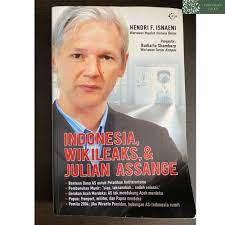
\includegraphics[width=0.85\textwidth]{../../images/python/page_016_img_04.jpeg}

\end{document}
